\documentclass{article}
\usepackage{tikz,amsmath,siunitx}
\usetikzlibrary{arrows,backgrounds,patterns,matrix,shapes,fit,calc,shadows,plotmarks}
\usetikzlibrary{positioning}
\usepackage[graphics,tightpage,active]{preview}
\PreviewEnvironment{tikzpicture}
\PreviewEnvironment{equation}
\PreviewEnvironment{equation*}
\newlength{\imagewidth}
\newlength{\imagescale}
\pagestyle{empty}
\thispagestyle{empty}

\begin{document}
    
	\begin{tikzpicture}[auto]
		\node[anchor=north west] (first normal)
			{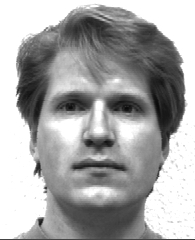
\includegraphics[] {s1-normal}};
		\node[right of=first normal,node distance=10cm] (first surprised) 	
			{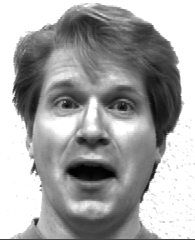
\includegraphics[] {s1-surprised}};
		\node[below of=first normal,node distance=10cm]  (second normal)
			{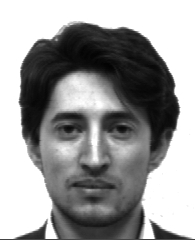
\includegraphics[] {s2-normal}};
		\node[right of=second normal,node distance=10cm]  (second surprised)
			{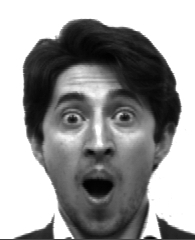
\includegraphics[] {s2-surprised}};	
			
%		\node[draw=blue!50, ultra thick, line join=round, fit=(first normal) (first surprised)] {};
%		\node[draw=blue!50, ultra thick, line join=round, fit=(second normal) (second surprised)] {};
		
		\node[draw=green!50, ultra thick, line join=round, fit=(first normal) (second normal)] {};
		\node[draw=green!50, ultra thick, line join=round, fit=(first surprised) (second surprised)] {};
%		
%		\node[below left of=second surprised, node distance=7cm] (text) 
%			{\LARGE Face recognition};
	\end{tikzpicture}
	
\end{document}

















